\documentclass[12pt]{book}
\usepackage[utf8]{inputenc}
\usepackage[T1]{fontenc}
\usepackage{mathptmx}
\usepackage{geometry}
\usepackage{mathtools}
\usepackage[english]{babel}
\usepackage{graphicx}
\usepackage{subcaption}
\usepackage{stackengine}
\usepackage[os=win]{menukeys}
\usepackage{hyperref}
\usepackage{xcolor}
\usepackage{tikz}
\usepackage[yyyymmdd,hhmmss]{datetime}
\usepackage{etoolbox}
\usepackage[inline]{enumitem}
\usepackage{listings}
\usepackage{pdfpages}

\newcommand{\WindowsLogo}{\raisebox{-0.1em}{
\includegraphics[height=0.8em]{images/logo/Windows_3_logo_simplified}}}
%\newcommand{\PowerLogo}{\raisebox{-0.1em}{
\includegraphics[height=0.8em]{images/logo/power}}}
\newcommand{\WinKey}{\keys{\WindowsLogo}}
\newcommand{\PowerKey}{\keys{\PowerLogo}}

\patchcmd{\thebibliography}{\section*{\refname}}{}{}{}

\addto\captionsenglish{\renewcommand{\contentsname}{Daftar Isi}}
\addto\captionsenglish{\renewcommand{\figurename}{Gambar}}

\hypersetup{
	colorlinks=true, %set true if you want colored links
	linktoc=all,     %set to all if you want both sections and subsections linked
	linkcolor=blue,  %choose some color if you want links to stand out
	urlcolor=blue,   %url color
}

\geometry{
	a4paper,
	left=10mm,
	right=10mm,
	top=15mm,
	bottom=15mm,
}

\date{}

\hypersetup{citecolor=black}

\definecolor{LightGray}{gray}{0.95}

%\pagecolor[rgb]{0.1,0.1,0.1}
%\color[rgb]{1,1,1}

\lstset
{
	language=bash,
	breaklines=true,
	basicstyle=\tt\normalsize,
	frame = single
}

\begin{document}

	\frontmatter
	\begin{titlepage}
		\centering
		{\LARGE \bf Panduan Dasar Draft PCB Menggunakan KiCAD}
		\vfill
		{\Large Achmadi ST MT}
		\vfill
		
\includegraphics[width=250pt]{images/logo/logoviblab}
		\vfill
		\vfill
	\end{titlepage}

	%%%%%%%%%%%%%%%%%%%%%%%%%%%%%%%%%%%%%%%%%%%%%%%%%%%%%%%%%%%%%%%%%

	\newpage
	\tableofcontents

	%%%%%%%%%%%%%%%%%%%%%%%%%%%%%%%%%%%%%%%%%%%%%%%%%%%%%%%%%%%%%%%%%

	%%%%%%%%%%%%%%%%%%%%%%%%%%%%%%%%%%%%%%%%%%%%%%%%%%%%%%%%%%%%%%%%%

	\newpage
	\chapter{Penggunaan Buku}

	\section{Umum}
	Buku ini dibuat dengan tujuan penggunaan utama sebagai panduan digital untuk mempermudah search dan copy-paste.
	Anda tidak perlu mencetak buku ini ke bentuk kertas.
	Seluruh navigasi buku ini diharapkan menggunakan klik ke hyperlink di Daftar Isi,
	atau menggunakan tampilan \textbf{Index} yang tersedia di \textbf{SideBar} program pembaca PDF yang anda gunakan.

	\section{Petunjuk}
	Beberapa petunjuk yang digunakan di buku ini:
	\begin{itemize}
		\item \textbf{Cetak Tebal}: Menginformasikan identifier (keyword, variabel, fungsi, alamat, nama file, dst) yang berada di suatu paragraf
		\item \textit{Cetak Miring}: Bersama simbol panah (->) dan simbol lain, menginformasikan langkah-langkah klik menu/tombol.
		\item \textbf{TIPS:} Menginformasikan hal-hal yang dapat membantu atau pengetahuan tambahan.
		\item \textbf{PERINGATAN:} Menginformasikan hal-hal yang bener-benar harus diperhatikan.
	\end{itemize}

	%%%%%%%%%%%%%%%%%%%%%%%%%%%%%%%%%%%%%%%%%%%%%%%%%%%%%%%%%%%%%%%%%

	\newpage
	\mainmatter
	\chapter{Program KiCAD}

	\section{Pengenalan}

	KiCAD adalah paket software EDA (Electronic Design Automation) yang dikembangkan untuk perancangan papan sirkuit elektronik tercetak (Printed Circuit Board atau PCB)
	secara professional yang bersifat gratis dan terbuka.

	KiCAD dapat disandingkan dengan perangkat perancangan PCB professional lain seperti Altium, Diptrace, EasyEDA, dan lainnya.
	KiCAD tersedia untuk sistem operasi Windows, GNU/Linux, dan MacOS.\\

	Berikut adalah tampilan 4 software utama dalam paket software KiCAD:
	\begin{figure}[!ht]
		\centering
		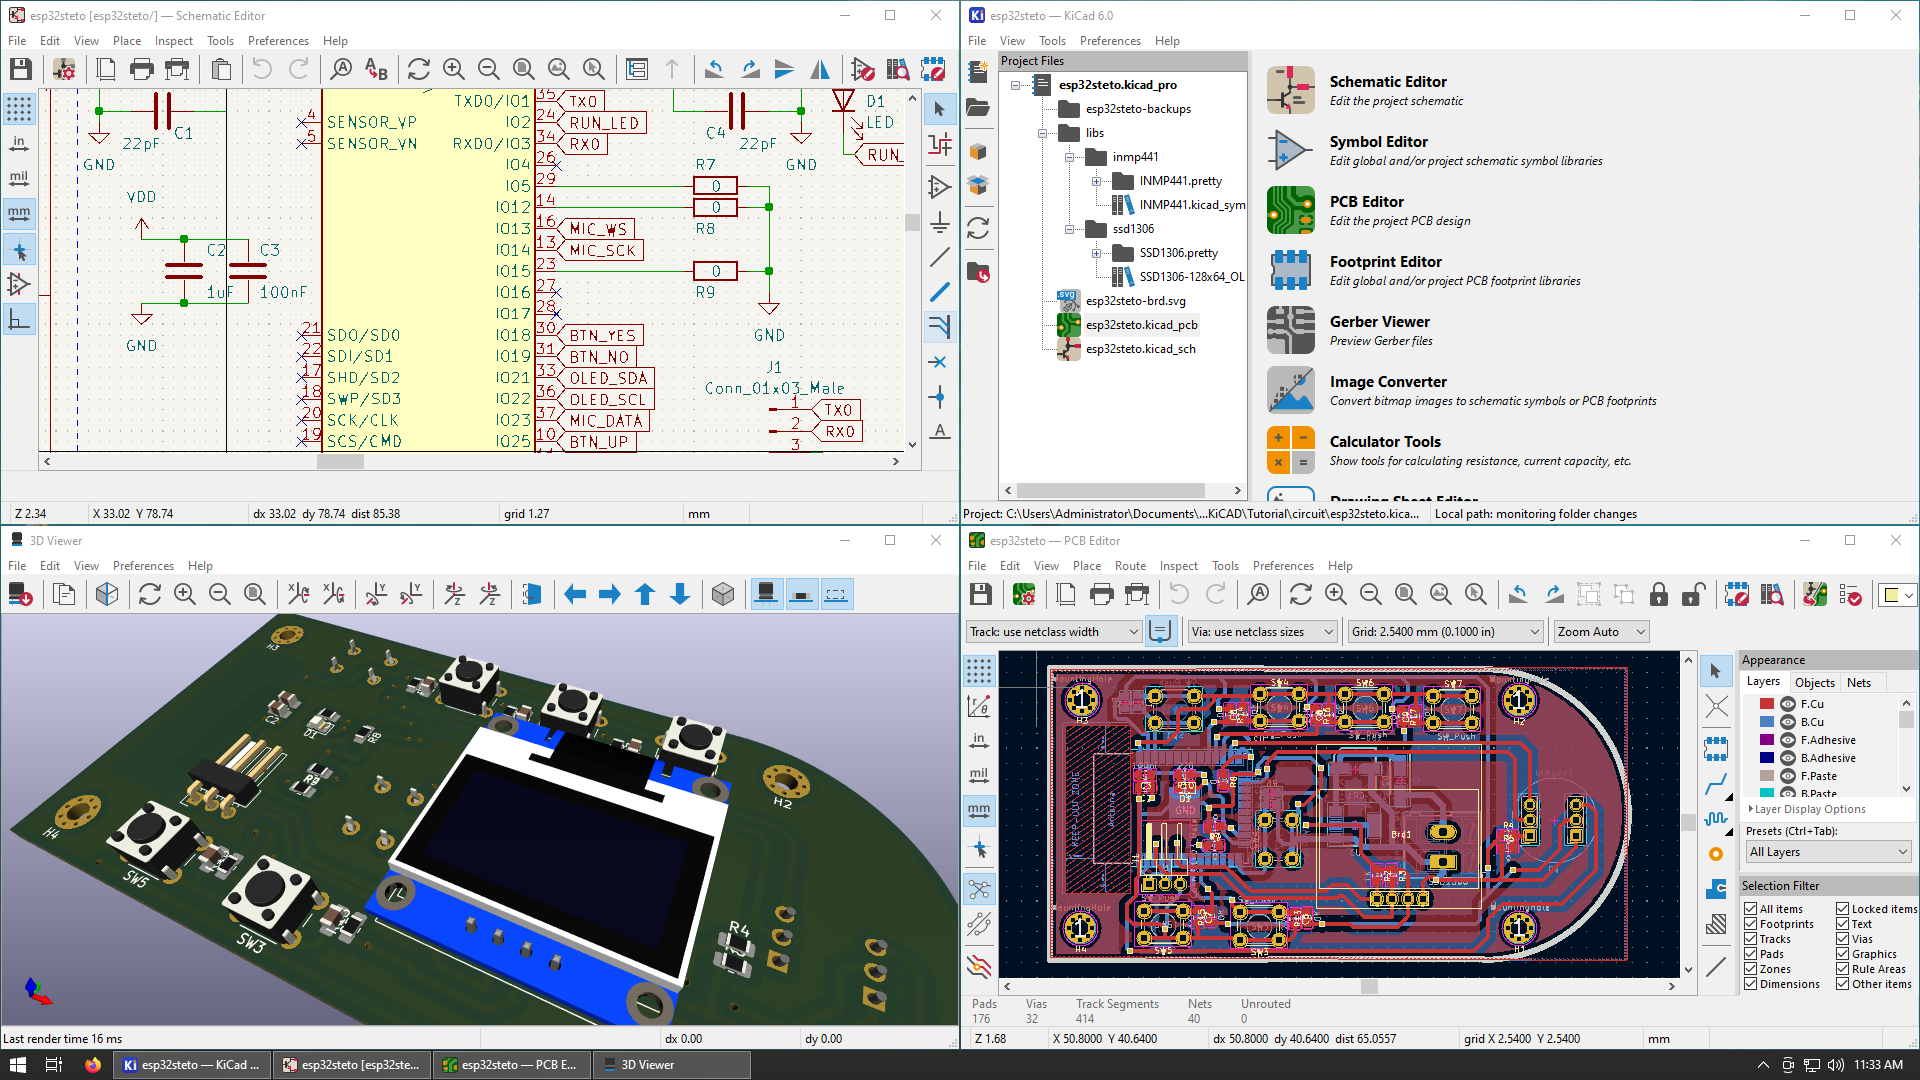
\includegraphics[width=\textwidth]{images/kicad_windows10}
		\caption{Tampilan KiCAD Windows 10}
	\end{figure}

	\textbf{TIPS:} Sepanjang tutorial, akan digunakan tampilan Windows 10 atau GNU/Linux sebagai acuan.
	Namun tutorial yang sama akan dapat pula digunakan di sistem operasi lain seperti Windows 8 dan Windows 11.\\

	\textbf{PERINGATAN:} Versi KiCAD yang akan digunakan adalah versi 6, dimana untuk sistem operasi Windows
	hanya bisa diinstal di Windows 8 dan selanjutnya.
	Untuk pengguna Windows 7 dan sebelumnya, disarankan menggunakan KiCAD versi 5.

	\newpage
	\section{Instalasi}

	\subsection{GNU/Linux}

	Berikut panduan instalasi KiCAD untuk dua jenis GNU/Linux yang populer, yaitu:
	\begin{itemize}
		\item Arch based, seperti Arch-Linux dan Manjaro.
		\item Ubuntu based, seperti Ubuntu-Mate dan Xubuntu.
	\end{itemize}

	\textbf{TIPS:} Untuk sistem operasi GNU/Linux, semua instalasi dilakukan via perintah di
	terminal emulator dengan sumber paket instalasi adalah mirror terdekat dari repository server masing-masing sistem operasi.\\

	\textbf{TIPS:} Perlu diingat untuk instalasi di GNU/Linux dibutuhkan hak akses administratif (umumnya sudo),
	sehingga dibutuhkan password akses tersebut.

	\subsubsection{Arch based}

	Untuk instalasi software KiCAD dan pustaka dasar, perintahnya adalah:

	\begin{lstlisting}
sudo pacman -S kicad kicad-library
	\end{lstlisting}

	Ukuran download berkisar 70MB dan ukuran instalasi berkisar 400MB.\\

	Kemudian untuk instalasi pustaka model komponen 3D, perintahnya adalah:

	\begin{lstlisting}
sudo pacman -S kicad-library-3d
	\end{lstlisting}

	Ukuran download berkisar 350Mb dan ukuran instalasi berkisar 5GB.\\

	\textbf{TIPS:} Jika diperlukan, lakukan update/upgrade sistem operasi dengan perintah:

	\begin{lstlisting}
sudo pacman -Syu --noconfirm
	\end{lstlisting}

	\subsubsection{Ubuntu based}

	Untuk instalasi KiCAD pada sistem operasi ini, digunakan sumber PPA khusus KiCAD 6:\\
	\url{https://launchpad.net/~kicad/+archive/ubuntu/kicad-6.0-releases} \\

	Pertama, tambahkan repository tersebut dengan perintah:
	\begin{lstlisting}
sudo add-apt-repository ppa:kicad/kicad-6.0-releases
sudo apt update
	\end{lstlisting}

	Kemudian perintah untuk instalasi seluruh paket lengkap (termasuk pustaka komponen 3D):
	\begin{lstlisting}
sudo apt install --install-recommends kicad
	\end{lstlisting}
	Ukuran download berkisar 500GB dan ukuran instalasi berkisar 6GB.\\

	Jika ingin menghindari paket komponen 3D dan menghemat ukuran instalasi, ganti perintah menjadi:

	\begin{lstlisting}
sudo apt install --install-recommends kicad kicad-library-packages3d-
	\end{lstlisting}

	\textbf{TIPS:} Jika memilih sistem operasi berbasis Ubuntu, disarankan memilih versi Ubuntu LTS dibandingkan
	reguler release.\\

	\textbf{PERINGATAN:} Hingga waktu penulisan tutorial ini, penulis hanya sebatas menggunakan
	KiCAD di Windows 10 dan Arch-Linux.
	Penulis belum mencoba pada sistem operasi Ubuntu.

	\newpage
	\subsection{Windows}

	Berikut panduan instalasi KiCAD untuk Windows 8, Windows 10, dan Windows 11.

	\subsubsection{Download}

	Installer KiCAD untuk Windows dapat didownload di alamat:\\
	\url{https://github.com/KiCad/kicad-source-mirror/releases}\\

	Atau spesifik untuk versi 6.0.7 untuk 64-bit dialamat:\\
	\url{https://github.com/KiCad/kicad-source-mirror/releases/download/6.0.7/kicad-6.0.7-x86_64.exe}\\

	\begin{figure}[!ht]
		\centering
		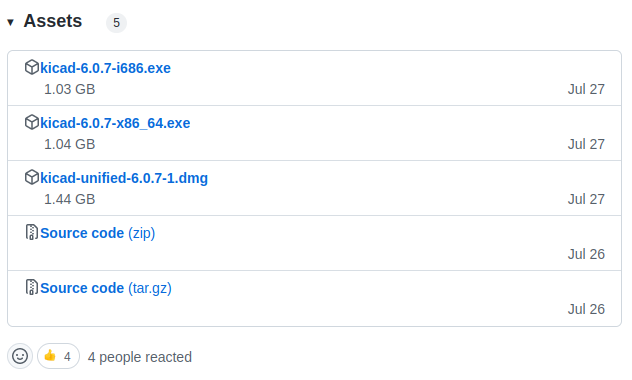
\includegraphics[width=0.75\textwidth]{images/installations/kicad_github}
		\caption{Download KiCAD}
	\end{figure}

	Ukuran berkas instalasi berkisar 1GB.\\

	\textbf{TIPS:} Penulis hanya merekomendasikan sumber instalasi dari URL Github di atas.
	Selain merupakan sumber resmi, juga Github menyediakan kecepatan download cukup tinggi.\\

	\textbf{TIPS:} Jika dibutuhkan versi 5 (seperti untuk Windows 7), dapat dikunjungi alamat berikut:\\
	\url{https://downloads.kicad.org/kicad/windows/explore/stable}\\

	Tutorial ini hanya akan menjelaskan KiCAD versi 6.

	\newpage
	\subsubsection{Proses Instalasi}

	Jalankan program installer yang telah di didownload. Klik \textit{Next}

	\begin{figure}[!ht]
		\centering
		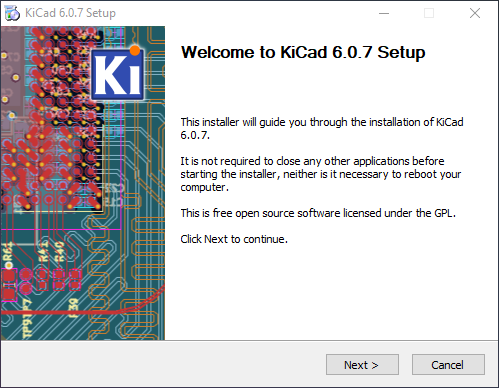
\includegraphics[width=0.7\textwidth]{images/installations/kicad_install_0}
		\caption{Memulai Instalasi KiCAD}
	\end{figure}

	Pilih paket apa saja yang ingin diinstal.
	Disini dapat di-\textit{unselect} paket Footprint 3D jika ada ingin menghemat 5GB instalasi.
	Lanjut klik \textit{Next}

	\begin{figure}[!ht]
		\centering
		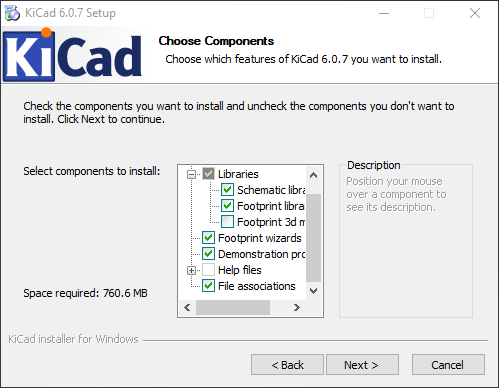
\includegraphics[width=0.7\textwidth]{images/installations/kicad_install_1}
		\caption{Pilih Paket}
	\end{figure}

	\newpage
	Tunggu proses instalasi hingga selesai

	\begin{figure}[!ht]
		\centering
		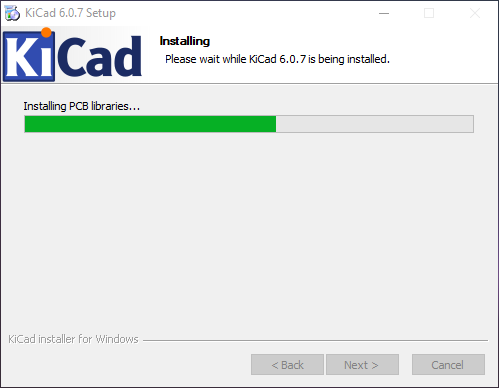
\includegraphics[width=0.7\textwidth]{images/installations/kicad_install_2}
		\caption{Proses Instalasi}
	\end{figure}

	Setelah instalasi selesai, dapat diklik \textit{Finish}.
	Tidak perlu install FreeCAD untuk saat ini.

	\begin{figure}[!ht]
		\centering
		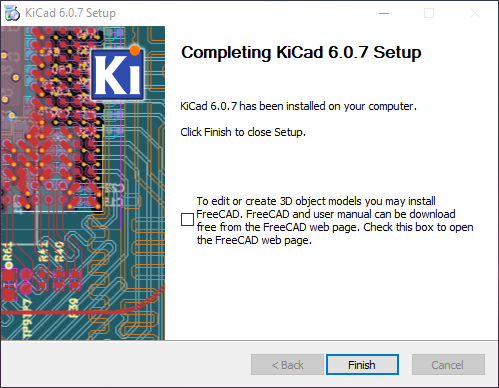
\includegraphics[width=0.7\textwidth]{images/installations/kicad_install_3}
		\caption{Instalasi Selesai}
	\end{figure}

	\newpage
	\subsection{MacOS}
	Nanti akan dilengkapi saat penulis cukup berduit untuk memiliki laptop Apple dan MacOS.

	\section{Memulai Program}

	Untuk memulai program KiCAD pada GNU/Linux, dapat digunakan perintah:
	\begin{lstlisting}
kicad
	\end{lstlisting}

	Atau dapat pula melalui menu sistem seperti pada sistem operasi Windows

	\begin{figure}[!ht]
		\centering
		\begin{subfigure}[t]{0.4\textwidth}
			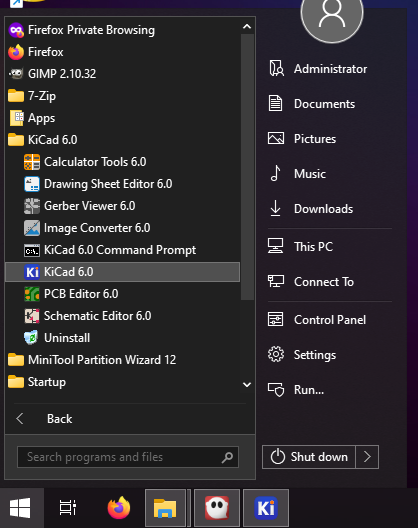
\includegraphics[width=\textwidth]{images/installations/kicad_menu_all}
			\caption{Windows 10}
		\end{subfigure}
		\begin{subfigure}[t]{0.4\textwidth}
			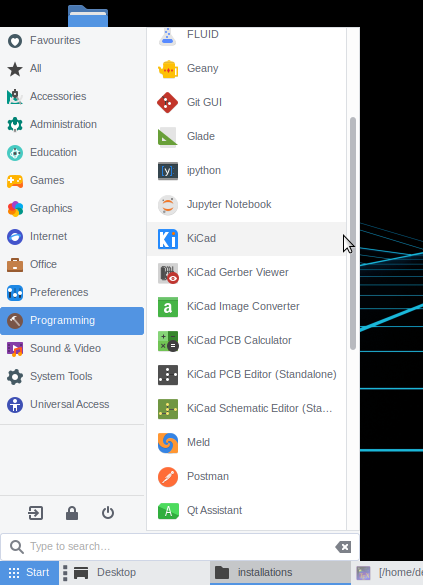
\includegraphics[width=\textwidth]{images/installations/kicad_menu_linux}
			\caption{Arch Linux}
		\end{subfigure}
		\caption{Memulai KiCAD via menu sistem operasi}
	\end{figure}

	Jika instalasi sukses, akan tampil pilihan migrasi pengaturan.
	Pilih default saja dan klik \textit{OK}.

	\begin{figure}[!ht]
		\centering
		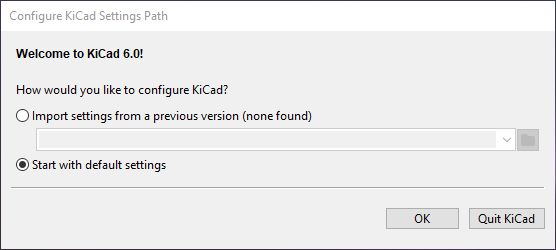
\includegraphics[width=0.7\textwidth]{images/installations/kicad_welcome}
		\caption{Migrasi Pengaturan}
	\end{figure}

	\newpage
	Tunggu beberapa saat, maka program utama KiCAD akan muncul.

	\begin{figure}[!ht]
		\centering
		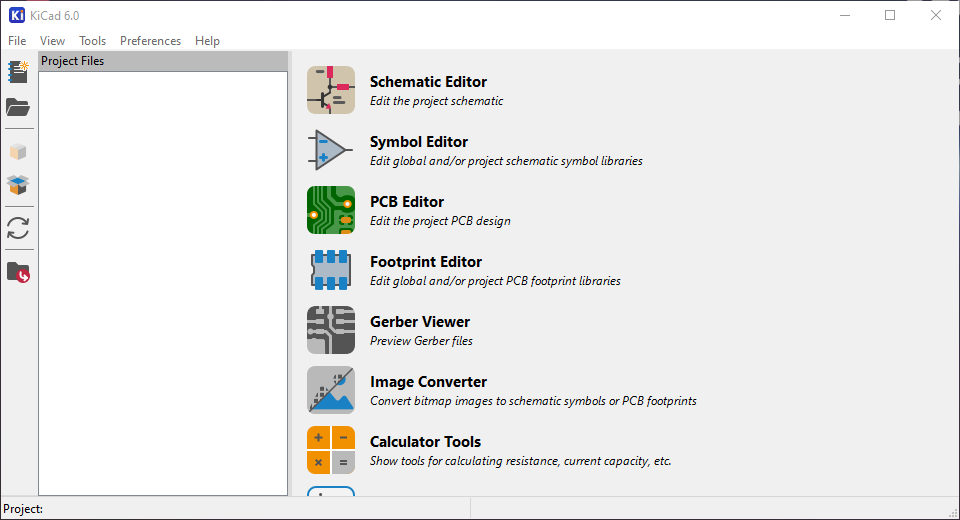
\includegraphics[width=\textwidth]{images/installations/kicad_first}
		\caption{Program Utama KiCAD}
	\end{figure}

	\textbf{PERINGATAN:} Jika saat menjalankan KiCAD muncul pesan OpenGL error seperti di bawah ini:

	\begin{figure}[!ht]
		\centering
		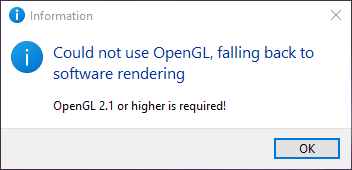
\includegraphics[width=0.7\textwidth]{images/installations/kicad_warn_noopengl}
		\caption{Peringatan OpenGL}
	\end{figure}

	Maka besar kemungkinan driver display atau VGA komputer masih menggunakan driver bawaan Windows.
	Silahkan update driver display komputer anda sesuai hardware yang terpasang.\\


	\centering \textbf{Sampai disini, proses instalasi telah selesai.}

\end{document}